\documentclass[12pt]{article}

\usepackage{amssymb, amsmath, amsfonts}
\usepackage{mathtools}
\usepackage{amsthm}
\usepackage{moreverb}
\usepackage{graphicx}
\usepackage{enumerate}
\usepackage{graphics}
\usepackage{color}
\usepackage{array}
\usepackage{float}
\usepackage{hyperref}
\usepackage{textcomp}
\usepackage{alltt}
\usepackage{mathtools}
\usepackage[T1]{fontenc}
\usepackage{ulem}
\usepackage{fullpage}
\usepackage{tikz}
\usepackage{pgfplots}
\usepackage[utf8]{inputenc}
\newcommand{\suchthat}{\, \mid \,}
\allowdisplaybreaks
\def\arraystretch{1.3}

\begin{document}

{\bf MATH 481A \hfill Numerical Analysis \ \ \ \ \ \hfill Spring 2015}

\title{\bf Hw \# 3 Solutions}
\author{\bf Sam Fleischer}
\date{\bf Tues. Mar. 10, 2015}

{\let\newpage\relax\maketitle}
\maketitle
\tableofcontents
\pagebreak

\section*{Chapter 10}
\addcontentsline{toc}{section}{Chapter 10}

\subsection*{Section 10.10}
\addcontentsline{toc}{subsection}{Section 10.10}

\subsubsection*{34.}
\addcontentsline{toc}{subsubsection}{34}
{\it Suppose that the equation $f(x) = x^2 + a_1x + a_2 = 0$ possesses real roots $\alpha$ and $\beta$.  Show that the iteration $z_{k+1} = -\dfrac{a_1z_k + a_2}{z_k}$ is stable at $x = \alpha$ if $|\alpha| > |\beta|$, the iteration $z_{k+1} = -\dfrac{a_2}{z_k + a_1}$ is stable at $x = \alpha$ if $|\alpha| < |\beta|$, and the iteration $z_{k+1} = -\dfrac{z_k^2 + a_2}{a_1}$ is stable at $x = \alpha$ if $2|\alpha| < |\alpha + \beta|$.}

\noindent Suppose $\alpha$ and $\beta$ are the roots of $f(x) = 0$ such that $\alpha > \beta$.  We know that $\alpha + \beta = -a_1$ and $\alpha\beta = a_2$.  We can rearrange $f(x) = 0$ to be $x = F(x)$ in the following ways:
\begin{enumerate}[\ \ 1)\ \ ]
\item $x = F_1(x) = -\dfrac{a_1x + a_2}{x}$.  The iterative method that arises from this is $z_{k+1} = -\dfrac{a_1z_k + a_2}{z_k}$.  But $F_1'(x)  = \dfrac{a_2}{x^2} = \dfrac{\alpha\beta}{x^2}$.  If $|\alpha| > |\beta|$, then $\left|\dfrac{\beta}{\alpha}\right| < 1$.  But $|F_1'(\alpha)| = \left|\dfrac{\beta}{\alpha}\right| < 1$, proving the iterative method is stable.
\item $x = F_2(x) = -\dfrac{a_2}{x + a_1}$.  The iterative method that arises from this is $z_{k+1} = -\dfrac{a_2}{z_k + a_1}$.  But $F_2'(x)  = \dfrac{a_2}{(x+a_1)^2} = \dfrac{\alpha\beta}{(x - \alpha - \beta)^2}$.  If $|\alpha| < |\beta|$, then $\left|\dfrac{\alpha}{\beta}\right| < 1$.  But $|F_2'(\alpha)| = \left|\dfrac{\alpha}{\beta}\right| < 1$, proving the iterative method is stable.
\item $x = F_3(x) = -\dfrac{x^2 + a_2}{a_1}$.  The iterative method that arises from this is $z_{k+1} = -\dfrac{z_k^2 + a_2}{a_1}$.  But $F_3'(x)  = -\dfrac{2x}{a_1} = \dfrac{2x}{\alpha + \beta}$.  If $2|\alpha| < |\alpha + \beta|$, then $\left|\dfrac{2\alpha}{\alpha + \beta}\right| < 1$.  But $|F_3'(\alpha)| = \left|\dfrac{2\alpha}{\alpha + \beta}\right| < 1$, proving the iterative method is stable.
\end{enumerate}

\subsubsection*{37.}
\addcontentsline{toc}{subsubsection}{37}
{\it The real root $\alpha$ of the equation $x + \log{x} = 0$ lies between $0.56$ and $0.57$.  Show that the iteration $z_{k+1} = -\log{z_k}$ is unstable at $x = \alpha$ and verify this fact by calculation.  Then show that the iteration $z_{k+1} = \exp[-z_k]$ is stable at $x = \alpha$, and determine $\alpha$ to five places.}

\noindent Let $F_1(x) = -\log{x}$, which produces the iterative method $z_{k+1} = -\log{z_k}$.  Note $F_1'(x) = -\dfrac{1}{x}$ and $|F_1'(\alpha)| > \dfrac{1}{0.57} > 1$, proving the iterative method is unstable.  However, set $F_2(x) = \exp{[-x]}$, which produces the iterative method $z_{k+1} = \exp[-z_k]$.  Note $F_2'(x) = -\exp{[-x]}$ and $|F_2'(\alpha)| < \exp{[-0.56]} < 1$, proving the iterative method is stable.  To compute the actual value of $\alpha$, I set $z_0 = 0.56$, and used Python to find the following values:
\begin{align*}
z_0 &= 0.56 \\
z_1 = \exp{[-z_0]} &= 0.571209063849 \\
z_2 = \exp{[-z_1]} &= 0.564842095522 \\
z_3 = \exp{[-z_2]} &= 0.568449900456 \\
z_4 = \exp{[-z_3]} &= 0.5664027392 \\
z_5 = \exp{[-z_4]} &= 0.567563444613 \\
z_6 = \exp{[-z_5]} &= 0.566905052824 \\
z_7 = \exp{[-z_6]} &= 0.567278421354 \\
z_8 = \exp{[-z_7]} &= 0.567066656979 \\
z_9 = \exp{[-z_8]} &= 0.567186754211 \\
z_{10} = \exp{[-z_9]} &= 0.567118640742 \\
z_{11} = \exp{[-z_{10}]} &= 0.567157270476 \\
z_{12} = \exp{[-z_{11}]} &= 0.567135361765 \\
z_{13} = \exp{[-z_{12}]} &= 0.567147787106 \\
z_{14} = \exp{[-z_{13}]} &= 0.567140740145 \\
z_{15} = \exp{[-z_{14}]} &= 0.567144736777 \\
z_{16} = \exp{[-z_{15}]} &= 0.567142470113 \\
z_{17} = \exp{[-z_{16}]} &= 0.567143755636 \\
z_{18} = \exp{[-z_{17}]} &= 0.56714302656 \\
\end{align*}
Clearly this is converging in an oscillatory fashion to $\boxed{\alpha \approx 0.567143}$.

\subsubsection*{40.}
\addcontentsline{toc}{subsubsection}{40}
{\it Consider the iterative solution of the equation $\tan{x} = x$.}
\begin{enumerate}[\it\ \ (a)\ \ ]
\item {\it By superimposing the graphs of $y=x$ and $y=\tan{x}$, show that the $r$\textsuperscript{th} positive root of this equation is in the interval $[r\pi, (r + \frac{1}{2})\pi]$.}\\
\centerline{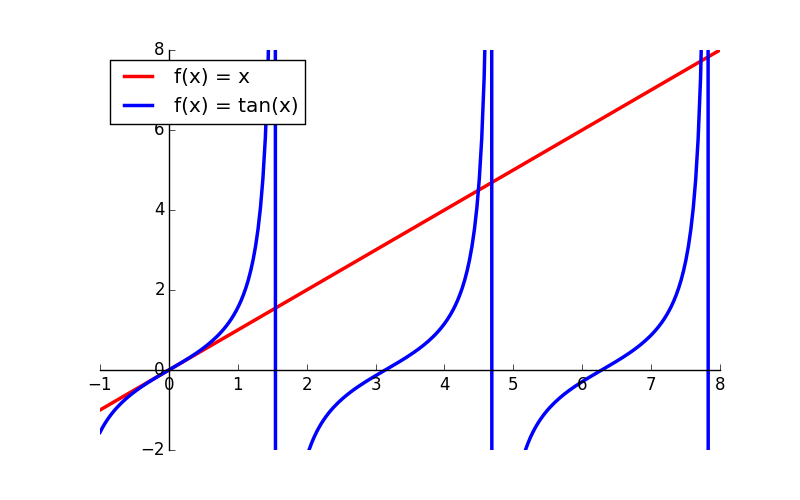
\includegraphics[scale=0.85]{tangent_graph.png}}
Clearly, the first intersection of $\tan{x}$ and $x$ occurs between $\pi$ and $(1 + \frac{1}{2})\pi$, and the second occurs between $2\pi$ and $(2 + \frac{1}{2})\pi$.  We can deduce that the $r$\textsuperscript{th} intersection occurs in the interval $[r\pi, (r + \frac{1}{2})\pi]$.

\item {\it Show that the iteration $z_{k+1} = r\pi + \tan^{-1}{z_k}$ is stable for the determination of the $r$\textsuperscript{th} positive root.}\\

\noindent Setting $F(x) = r\pi + \tan^{-1}{x}$ yields $F'(x) = \dfrac{1}{1 + x^2}$.  Since we are finding positive roots, we are only passing positive values to $F'(x)$, thus $F'(x) < 1\ \forall x > 0$, proving the iteration is stable for the $r$\textsuperscript{th} positive root.

\item {\it With $[a,b] = [r\pi, (r + \frac{1}{2})\pi]$ and $F(x) = r\pi + \tan^{-1}{x}$, show that when $a \leq x \leq b$ it is true that both $a < F(x) < b$ and $0 < F'(x) < 1$.  Hence deduce in two ways that convergence to $\alpha_r$ is assured if $a \leq z_0 \leq b$.}\\

\noindent Note that $F(x) = r\pi + \tan^{-1}{x}$ is an increasing function that thus reaches its minimum on $[a,b]$ at $a$ and its maximum at $b$.  Note $F(a) = r\pi + \tan^{-1}(a) = r\pi = a$ and $F(b) = r\pi + \tan^{-1}{b} < r\pi + \frac{1}{2}\pi = (r + \frac{1}{2})\pi = b$.  Thus $a < F(x) < b$.  Also, $F'(x) = \dfrac{1}{1 + x^2} < 1$ for $x > 0$.  Thus $0 < F'(x) < 1$.  Thus we know that convergence to $\alpha_r$ is assured if $a \leq z_0 \leq b$ in two ways.  On the one hand, we know the interval is contracting interval.  We also know that $|F'(x)| < 1$ for all values close to $\alpha_r$.

\item {\it Use the iteration of part (b) to determine both $\alpha_1$ and $\alpha_2$ to five decimal places.}\\

\noindent I used Python to compute the following:  set $z_0 = \pi$.  Then,
\begin{align*}
z_0 &= 3.14159 \\
z_1 = F(z_0) &= 4.40421966514 \\
z_2 = F(z_1) &= 4.48911944313 \\
z_3 = F(z_2) &= 4.49320682586 \\
z_4 = F(z_3) &= 4.4933998952 \\
z_5 = F(z_4) &= 4.49340900664 \\
z_6 = F(z_5) &= 4.49340943661
\end{align*}
Clearly, $\boxed{\alpha_1 \approx 4.49341}$.  I used Python to compute the following:  set $z_0 = 2\pi$.  Then,
\begin{align*}
z_0 &= 6.28318 \\
z_1 = F(z_0) &= 7.69615031257 \\
z_2 = F(z_1) &= 7.7247704596 \\
z_3 = F(z_2) &= 7.72524390334 \\
z_4 = F(z_3) &= 7.72525170619 \\
z_5 = F(z_4) &= 7.72525183478 \\
z_6 = F(z_5) &= 7.7252518369
\end{align*}
Clearly, $\boxed{\alpha_2 \approx 7.72525}$.
\end{enumerate}

\subsubsection*{41.}
\addcontentsline{toc}{subsubsection}{41}
{\it Consider the polynomial $f(x) = x^5 + 5x - 1$.}
\begin{enumerate}[\it\ \ (a)\ \ ]
\item {\it Prove that $f(x)$ has exactly one real zero $\alpha$ and that $0.1 < \alpha < 0.2$.}\\

\noindent Note $f'(x) = 5x^4 + 5$, which is positive for all $x$, and thus if there is a zero, there can only be one.  However, since $f$ is an odd-degree polynomial, it has an odd number of zeros.  Therefore, there is exactly one zero, $\alpha$.  Since $f(0.1) < 0$ and $f(0.2) > 0$, $\alpha \in (0.1, 0.2)$.

\item {\it Without more closely locating $\alpha$, prove that the iteration $z_{k+1} = z_k - cf(z_k)$ will converge to $\alpha$ if $0 < c < \frac{1}{5.008}$ and if $0.1 \leq z_0 \leq 0.2$.}\\

\noindent Suppose $F(x) = x - cf(x)$ and $z_0 \in [0.1, 0.2]$.  Then $F'(x) = 1 - cf'(x) = 1 - c(5x^4 + 5) < 1 - c(5(0.1)^4 + 5) = -5.0005c + 1$.  Thus $|F'(x)| < 1 \iff -1 < -5.0005c < 1 \iff 0 < c < \dfrac{2}{5.0005}$.  But $c < \dfrac{1}{5.008}$ certainly implies $c < \dfrac{2}{5.0005}$, and thus the iteration converges to $\alpha$.

\item {\it With the choice $c = \dfrac{1}{5.01}$, show that the asymptotic convergence factor is between $4 \times 10^{-4}$ and $2 \times 10^{-3}$, so that ultimately each iteration will provide three or four additional correct decimal places.}\\

\noindent For $c = \dfrac{1}{5.01}$, $F'(x) = 1 - \dfrac{1}{5.01}(5x^4 + 5)$.
\begin{align*}
F'(0.1) &= 1 - \dfrac{1}{5.01}(5.0005) \approx 1 - 0.99810379 \approx 0.0018962 \approx 2 \times 10^{-3} \\
F'(0.2) &= 1 - \dfrac{1}{5.01}(5.008) \approx 1 - 0.999600798 \approx 0.0003992 \approx 4\times 10^{-4}
\end{align*}
Since the asymptotic convergence factor $\rho_k$ is approximately $F'(\alpha)$ and $\alpha \in (0.1, 0.2)$, we deduce that $4 \times 10^{-4} < \rho_k < 2 \times 10^{-3}$, and thus each iteration will proved three or four additional correct decimal places.

\item {\it Verify that with $c = \dfrac{1}{5.01}$, two iterations provide 10-place accuracy when $z_0 = 0.2$, while three are needed when $z_0 = 0.1$.}\\

\noindent Using $z_{k+1} = z_k - cf(z_k)$ with $z_0 = 0.2$ yields the following:
\begin{align*}
z_0 &= 0.2 \\
z_1 = z_0 - \frac{1}{5.01}f(z_0) \approx 0.19993612774451097 \\
z_2 = z_1 - \frac{1}{5.01}f(z_1) \approx 0.199936102181 \\
z_3 = z_2 - \frac{1}{5.01}f(z_2) \approx 0.199936102171 \\
z_4 = z_3 - \frac{1}{5.01}f(z_3) \approx 0.199936102171 \\
\end{align*}
$z_2$ is accurate to 10 place values.  Using $z_{k+1} = z_k - cf(z_k)$ with $z_0 = 0.1$ yields the following:
\begin{align*}
z_0 &= 0.1 \\
z_1 = z_0 - \frac{1}{5.01}f(z_0) \approx 0.199798403194 \\
z_2 = z_1 - \frac{1}{5.01}f(z_1) \approx 0.199936046618 \\
z_3 = z_2 - \frac{1}{5.01}f(z_2) \approx 0.199936102149 \\
z_4 = z_3 - \frac{1}{5.01}f(z_3) \approx 0.199936102171 \\
z_5 = z_4 - \frac{1}{5.01}f(z_4) \approx 0.199936102171 \\
\end{align*}
$z_3$ is accurate to 10 place values.  Note we do not round the tenth value based on the eleventh value.  We truncate after 10 values.

\end{enumerate}

\subsection*{Section 10.11}
\addcontentsline{toc}{subsection}{Section 10.11}

\subsubsection*{46.}
\addcontentsline{toc}{subsubsection}{46}
{\it Repeat the determination of problems 37 \sout{and 38} using the Newton-Raphson iteration both with $f(x) = x + \log{x}$ and with $f(x) = x - e^{-x}$.}\\

\noindent The Newton-Raphson iterative method for $f(x) = 0$ is $z_{k+1} = z_k - \dfrac{f(z_k)}{f'(z_k)}$.  For $z_0 = 0.56$, and $f(x) = x + \log{x}$ \Big(and so $f'(x) = 1 + \dfrac{1}{x}$\Big), the following values are computed:
\begin{align*}
z_0 &= 0.56 \\
z_1 = z_0 - \frac{f(z_0)}{f'(z_0)} &= 0.567114331629 \\
z_2 = z_1 - \frac{f(z_1)}{f'(z_1)} &=  0.567143289938 \\
z_3 = z_2 - \frac{f(z_2)}{f'(z_2)} &=  0.56714329041 \\
z_4 = z_3 - \frac{f(z_3)}{f'(z_3)} &=  0.56714329041 \\
z_5 = z_4 - \frac{f(z_4)}{f'(z_4)} &=  0.56714329041
\end{align*}
This clearly converges much faster than the iterative method used in problem 37.  For $z_0 = 0.56$, and $f(x) = x - e^{-x}$ (and so $f'(x) = 1 + e^{-x}$), the following values are computed:
\begin{align*}
z_0 &= 0.56 \\
z_1 = z_0 - \frac{f(z_0)}{f'(z_0)} &= 0.567134037161 \\
z_2 = z_1 - \frac{f(z_1)}{f'(z_1)} &=  0.567143290394 \\
z_3 = z_2 - \frac{f(z_2)}{f'(z_2)} &=  0.56714329041 \\
z_4 = z_3 - \frac{f(z_3)}{f'(z_3)} &=  0.56714329041 \\
z_5 = z_4 - \frac{f(z_4)}{f'(z_4)} &=  0.56714329041
\end{align*}
This also clearly converges much faster than the iterative method used in problem 37.

\subsubsection*{48.}
\addcontentsline{toc}{subsubsection}{48}
{\it By applythin the Newton-Raphson procedure to $f(x) = 1 - \dfrac{1}{ax}$, obtain the recurrence formula $z_{k+1} = z_k(2 - az_k)$ for the iterative determination of the reciprocal of $a$ without effecting division, and show that if $\epsilon_k$ denotes the error in $z_k$, then there follows $\epsilon_{k+1} \approx a\epsilon_k^2$ when $z_k \approx \dfrac{1}{a}$.  Also show that the iteration will converge to $\dfrac{1}{a}$ if $0 < z_0 < \dfrac{2}{a}$.  Does it converge when $z_0 = 0$ or $z_0 = \dfrac{2}{a}$?}\\

\noindent Suppose $f(x) = 1 - \dfrac{1}{ax}$.  This clearly has one root, namely $\alpha = \dfrac{1}{a}$.  Also, $f'(x) = \dfrac{1}{ax^2}$.  Define a classical Newton-Raphson iterative method by $z_{k+1} = z_k - \dfrac{f(z_k)}{f'(z_k)}$.  Then
\begin{align*}
z_{k+1} = z_k - \dfrac{f(z_k)}{f'(z_k)} = z_k - \dfrac{1 - \dfrac{1}{az_k}}{\dfrac{1}{az_k^2}} = z_k - (az_k^2 - z_k) = z_k(2 - az_k)
\end{align*}
Let $\epsilon_k$ denote the error of $z_k$, that is, $|\alpha - z_k|$, or $\left|\dfrac{1}{a} - z_k\right|$.  Then
\begin{align*}
\epsilon_{k+1} = |\alpha - z_{k+1}| = |\alpha - z_k(2 - az_k)| = |a(\alpha^2 - 2\alpha z_k + z_k^2)| = |a(\alpha - z_k)^2| = a\epsilon_k^2
\end{align*}
Pick $z_0$ such that $0 < z_0 < \dfrac{2}{a}$.  Then $|z_0 - \alpha| < \alpha$.  Thus since $\epsilon_{k+1} = a\epsilon_k^2$,
\begin{align*}
|\alpha - z_1| &= a(\alpha - z_0)^2 < a\alpha^2 = \alpha \\
\implies |\alpha - z_2| &= a(\alpha - z_1)^2 < a\alpha^2 = \alpha \\
&\ \ \vdots \\
\implies |\alpha - z_{k+1}| &= a(\alpha - z_k)^2 < a\alpha^2 = \alpha 
\end{align*}
Thus the iterative method $F(x) = x - \dfrac{f(x)}{f'(x)}$ is a contractive mapping on $(0, 2\alpha)$, and thus converges to $\alpha$ for any $z_0 \in (0, 2\alpha)$.  Since $f$ and $f'$ are undefined at $0$, we can say that this iteration does not converge for $z_0 = 0$.  Note $F(2\alpha) = 2\alpha(2 - a(2\alpha)) = 2\alpha\cdot(0) = 0$.  Then the iteration diverges, and so this iteration does not converge for $z_0 = 2\alpha$.

\subsubsection*{55.}
\addcontentsline{toc}{subsubsection}{55}

{\it Suppose that $f(x)$ possesses two zeros $\alpha_1$ and $\alpha_2$ which are nearly coincident, so that $f'(x)$ vanishes at a point $\beta$ between $\alpha_1$ and $\alpha_2$.  By making use of the relation}
\begin{align*}
f(\alpha) = f(\beta) + (\alpha - \beta)f'(\beta) + \dfrac{(\alpha - \beta)^2}{2}f''(\beta) + \dots
\end{align*}
{\it show that if $\beta$ is determined first, then initial approximations to the nearby zeros of $f(x)$ are given by}
\begin{align*}
\alpha_{1,2} \approx \beta \pm \left[-\dfrac{2f(\beta)}{f''(\beta)}\right]^{\frac{1}{2}}
\end{align*}
{\it if $f''(\beta) \neq 0$, and are real if $f(\beta)$ and $f''(\beta)$ are of opposite sign, after which improved values may be obtained by an appropriate iterative method.  [Note that the case of a double root $\alpha$ is also included since then $f(\beta) = 0$ and $\beta = \alpha$.]  Also use this procedure to determine the two real roots of the equation
\begin{align*}
3x^4 + 8x^3 - 6x^2 - 25x + 19 = 0
\end{align*}
(which are near $x = 1$) to five places.}\\

\noindent Supposing $f(x)$ has two real zeros $\alpha_1$ and $\alpha_2$ which are nearly coincident so that $f'(\beta) = 0$ for some $\beta \in [\alpha_1, \alpha_2]$, then we can use the following relation to determine $\alpha_1$ and $\alpha_2$.
\begin{align*}
f(\alpha) \approx f(\beta) + (\alpha - \beta)f'(\beta) + \dfrac{(\alpha - \beta)^2}{2}f''(\beta)
\end{align*}
Since $f'(\beta) = 0$ and $f(\alpha) = 0$, 
\begin{align*}
0 &\approx f(\beta) + \frac{(\alpha - \beta)^2}{2}f''(\beta) \\
&\approx \left(\frac{f''(\beta)}{2}\right)\alpha^2 + \left(-\beta f''(\beta)\right)\alpha + \left(f(\beta) + \frac{\beta^2f''(\beta)}{2}\right) \\
\implies \alpha_{1,2} &\approx \frac{\beta f''(\beta) \pm \sqrt{\beta^2\left[f''(\beta)\right]^2 - 2f(\beta)f''(\beta) - \beta^2\left[f''(\beta)\right]^2}}{f''(\beta)} \\
&\approx \beta \pm \sqrt{-2\frac{f(\beta)}{f''(\beta)}}
\end{align*}
This is only true if $f''(x) \neq 0$ and if $f(\beta)$ and $f''(\beta)$ are of opposite sign.  Now consider
\begin{align*}
f(x) &= 3x^4 + 8x^3 - 6x^2 - 25x + 19 = 0 \\
f'(x) &= 12x^3 + 24x^2 - 12x - 25 \\
f''(x) &= 36x^2 + 48x - 12
\end{align*}
and note that $f'(x)$ has a zero near $x = 1$.  Then let $\beta = 1$, and so $f(\beta) = -1$ and $f''(\beta) = 72 \neq 0$.  We can use the previous result since $f(\beta)$ and $f''(\beta)$ are of opposite sign.  So,
\begin{align*}
\alpha_{1,2} &\approx 1 \pm \sqrt{-2\cdot \frac{-1}{72}} \\
&\approx 1 \pm \frac{1}{6} \approx 0.8\overline{3} \text{ and } 1.1\overline{6
}\end{align*}
Using the Newton-Raphson iterative method, $z_{k+1} = z_k - \dfrac{f(z_k)}{f'(z_k)}$, with $z_0 = 0.833$, we attain
\begin{align*}
z_0 &= 0.833 \\
z_1 = z_0 - \frac{f(z_0)}{f'(z_0)} &= 0.840030007503 \\
z_2 = z_1 - \frac{f(z_1)}{f'(z_1)} &=  0.840149213603 \\
z_3 = z_2 - \frac{f(z_2)}{f'(z_2)} &=  0.840149248228 \\
z_4 = z_3 - \frac{f(z_3)}{f'(z_3)} &=  0.840149248228 \\
z_5 = z_4 - \frac{f(z_4)}{f'(z_4)} &=  0.840149248228
\end{align*}
Thus $\alpha_1 \approx 0.840149$.  Using the Newton-Raphson iterative method, $z_{k+1} = z_k - \dfrac{f(z_k)}{f'(z_k)}$, with $z_0 = 1.167$, we attain
\begin{align*}
z_0 &= 1.167 \\
z_1 = z_0 - \frac{f(z_0)}{f'(z_0)} &= 1.17229382387 \\
z_2 = z_1 - \frac{f(z_1)}{f'(z_1)} &=  1.17219516283 \\
z_3 = z_2 - \frac{f(z_2)}{f'(z_2)} &=  1.17219512836 \\
z_4 = z_3 - \frac{f(z_3)}{f'(z_3)} &=  1.17219512836 \\
z_5 = z_4 - \frac{f(z_4)}{f'(z_4)} &=  1.17219512836
\end{align*}
Thus $\alpha_2 \approx 1.172195$.

\subsubsection*{57.}
\addcontentsline{toc}{subsubsection}{57}

{\it Proceed as in problem 55 with the root pair of the equation}
\begin{align*}
f(x) = x^6 - 16x^3 + x^2 + 59 = 0
\end{align*}
{\it which is near $x = 2$.} \\

\noindent Note the following:
\begin{align*}
f'(x) &= 6x^5 - 48x^2 + 2x \\
f''(x) &= 30x^4 - 96x + 2
\end{align*}
Note $f'(x)$ has a zero near $x = 2$, so let $\beta = 2$.  Then $f(\beta) = -1< 0$ and $f''(\beta) = 290 > 0$.  We can use the previous result since $f(\beta)$ and $f''(\beta)$ are of opposite sign.  So,
\begin{align*}
\alpha_{1,2} &\approx 2 \pm \sqrt{-2\cdot \frac{-1}{290}} \\
&\approx 2 \pm \frac{1}{12} \approx 1.91\overline{6} \text{ and } 2.08\overline{3}\end{align*}
Using the Newton-Raphson iterative method, $z_{k+1} = z_k - \dfrac{f(z_k)}{f'(z_k)}$, with $z_0 = 1.9167$, we attain
\begin{align*}
z_0 &= 1.9167 \\
z_1 = z_0 - \frac{f(z_0)}{f'(z_0)} &= 1.89314133146 \\
z_2 = z_1 - \frac{f(z_1)}{f'(z_1)} &=  1.895837569 \\
z_3 = z_2 - \frac{f(z_2)}{f'(z_2)} &=  1.89587198372 \\
z_4 = z_3 - \frac{f(z_3)}{f'(z_3)} &=  1.89587198937 \\
z_5 = z_4 - \frac{f(z_4)}{f'(z_4)} &=  1.89587198937 \\
z_6 = z_5 - \frac{f(z_5)}{f'(z_5)} &=  1.89587198937
\end{align*}
Thus $\alpha_1 \approx 1.89587$.  Using the Newton-Raphson iterative method, $z_{k+1} = z_k - \dfrac{f(z_k)}{f'(z_k)}$, with $z_0 = 2.083$, we attain
\begin{align*}
z_0 &= 2.083 \\
z_1 = z_0 - \frac{f(z_0)}{f'(z_0)} &= 2.06965633786 \\
z_2 = z_1 - \frac{f(z_1)}{f'(z_1)} &=  2.06843314443 \\
z_3 = z_2 - \frac{f(z_2)}{f'(z_2)} &=  2.06842295626 \\
z_4 = z_3 - \frac{f(z_3)}{f'(z_3)} &=  2.06842295555 \\
z_5 = z_4 - \frac{f(z_4)}{f'(z_4)} &=  2.06842295555 \\
z_6 = z_5 - \frac{f(z_5)}{f'(z_5)} &=  2.06842295555
\end{align*}
Thus $\alpha_2 \approx 2.068423$.


%\pagebreak
%\begin{thebibliography}{99}
%
%\bibitem{Abrams1997b}
%Abrams, P.~A. and Matsuda, H.
%Prey Adaptation as a Cause of Predator-Prey Cycles.
%\emph{Evolution}
%1997, 51:1742-1750.
%
%\bibitem{Chavez2001}
%Brauer, F., Castillo-Chavez, C.
%Mathematical Models in Population Biology and Epidemiology.
%Springer,
%2011. Print.
%
%\bibitem{Boyce2012}
%Boyce, W. E., and DiPrima, R. C.
%Elementary Differential Equations and Boundary Value Problems %10\textsuperscript{th} ed.
%Wiley Global Education
%2012. Print.
%
%\bibitem{Saloniemi1993}
%Saloniemi, I.
%A Coevolutionary Predator-Prey Model with Quantitative Characters.
%\emph{American Naturalist}
%1993, 141:880-896.
%
%\bibitem{Schreiber2011}
%Schreiber, S.~J., B$\ddot{\mbox{u}}$rger,  R., and Bolnick,  D.~I.
%The Community Effects of Phenotypic and Genetic Variation within a Predator %Population.
%\emph{Ecology}
%2011,  92(8):526-543. 
%
%\end{thebibliography}

\end{document}